\documentclass[11pt, oneside, draft]{article} 
\usepackage[utf8]{inputenc} 
\usepackage{a4wide} 
\usepackage[russian]{babel} 
\usepackage{graphicx} 
\usepackage{epstopdf} 
\usepackage{amsmath} 
\usepackage{amsfonts} 
\usepackage{amssymb} 
\usepackage{amsthm}
\usepackage[perpage]{footmisc}
%\newtheoremstyle{mytheorem}% name of the style to be used
%  {}% measure of space to leave above the theorem. E.g.: 3pt
%  {}% measure of space to leave below the theorem. E.g.: 3pt
%  {}% name of font to use in the body of the theorem
%  {}% measure of space to indent
%  {}% name of head font
%  {:}% punctuation between head and body
%  { }% space after theorem head; " " = normal interword space
%  {}% Manually specify head
%\theoremstyle{mytheorem}
\numberwithin{equation}{section} 
\newtheorem{definition}{Определение}[section] 
\newtheorem{theorem}{Теорема}[section] 
\newtheorem{property}{Свойство}[section] 
\newtheorem{corollary}{Следствие}[theorem] 
\newtheorem{lemma}[theorem]{Лемма} 
\newtheorem*{statement}{Утверждение} 
\renewenvironment{proof}{
\noindent\textit{Доказательство: }} {\qed}
\newcounter{icount}
\graphicspath{{figures/f1/}{figures/f2/}{figures/f3/}{figures/f4/}}
%commands
\newcommand \bitem[1][]{
\item \textbf{#1}} 
\newcommand \four[1][\lambda]{\mathfrak{F}(#1)} 
\newcommand \fft[1][\lambda]{F(#1)} 
\newcommand \rarrow{\rightarrow} 
\newcommand \intinf[1][{\,dt}]{ \int\limits_{-\infty}^{+\infty}{{#1}}} 
\renewcommand \qed{$\blacksquare$}

\DeclareMathOperator{\sgn}{sgn}

\begin{document}

%Title
    \thispagestyle{empty}
    \begin{center}
        \ \vspace{-3cm}
    
        
\includegraphics[width=0.5
        \textwidth]{msu}\\
        {\scshape Московский государственный университет имени М.~В.~Ломоносова}\\
        Факультет вычислительной математики и кибернетики\\
        Кафедра системного анализа
    
        \vfill
    
        {\LARGE Отчёт по практикуму}
    
        \vspace{1cm}
    
        {\Huge\bfseries "<Быстрое преобразование Фурье">} 
    \end{center}

    \vspace{1cm}
    \begin{flushright}
        \large \textit{Студент 315 группы}\\
        В.\,А.~Сливинский
    
        \vspace{5mm}
    
        \textit{Руководители практикума}\\
        к.ф.-м.н., доцент И.\,В.~Рублёв \\
        к.ф.-м.н., доцент П.\,А.~Точилин 
    \end{flushright}

    \vfill
    \begin{center}
        Москва, 2017 
    \end{center}
    \pagebreak

    %Contents
    \tableofcontents

    \pagebreak


    %Task

    \section{Постановка~задачи}

    \subsection{Общая~формулировка~задачи} Дана система функций (всюду далее, если не сказано противное, предполагается, что \(f(t) : \mathbb{R} \rightarrow \mathbb{R} \) и функция
    суммируема и обладает достаточной гладкостью) 
    \begin{equation}
        \label{functions} 
        \left\{ 
        \begin{aligned} 
            f_1(t) &= e^{-2|t|} \cos(t) \\
            f_2(t) &= \dfrac{e^{-|t|} - 1}{t} \\
            f_3(t) &= \dfrac{\arctg{t^2}}{1 + t^4} \\
            f_4(t) &= t^3e^{-t^4} 
       \end{aligned} 
       \right. 
    \end{equation} 
    Для каждой функции из системы \eqref{functions} требуется: \begin{enumerate} \item
    Получить аппроксимацию преобразования Фурье \( F(\lambda)\) для каждой функции \(f(t)\) из заданного набора при помощи быстрого преобразования Фурье ({\bfseries БПФ / FFT}),
    выбирая различные шаги дискретизации исходной функции и различные окна, ограничивающие область определения \(f(t)\) \item Построить графики \(F(\lambda)\) \item Для функций
    \(f_1(t)\) и \(f_2(t)\) из заданного набора вычислить аналитически преобразование Фурье \begin{equation}\label{fourier_transform} \boxed{\four = \intinf[{f(t) e^{-i\lambda t}\,
    dt}]} \end{equation} и сравнить графики \( \four \) с графиками \( F(\lambda)\), полученного из аппроксимации через {\bfseries БПФ}\\ \end{enumerate}
    %Formal task

    \subsection{Формальная~постановка~задачи} 
    \begin{enumerate}
        \item Реализовать на языке MATLAB функцию \\\texttt{plotFT(hFigure,~fHandle,~fFTHandle,~step,~inpLimVec,~outLimVec)} \\со следующими параметрами: 
        \begin{itemize}
            \bitem[hFigure] ~--- указатель на фигуру, в которой требуется отобразить графики \bitem[fHandle] ~--- указатель на функцию (\texttt{Function Handle}), которую требуется преобразовывать (\(f(t)\)) \bitem[fFTHandle] ~--- указатель на функцию (\texttt{Function Handle}), моделирующую аналитическое преобразование Фурье \eqref{fourier_transform} функции \(f(t)\) (может быть пустым вектором, в таком случае график аналитического преобразования строить не требуется) \bitem[step] ~--- положительное число, задающее шаг дискретизации \(\Delta t\) \bitem[inpLimVector] ~--- вектор-строка, задающая окно \([a, b]\) для функции \(f(t)\), первый элемент вектора содержит \(a\), второй \(b\), причём~\(a < b\), но не обязательно \(a = -b\) \bitem[outLimVector] ~--- вектор-строка, задающая окно \([c, d]\) \textit{для вывода} графика преобразования Фурье (пределы~осей~абсцисс). В случае, если передаётся пустой вектор, следует брать установленные в фигуре пределы или определять свои разумным образом 
        \end{itemize}
        Данная функция строит графики вещественной и мнимой частей численной аппроксимации преобразования Фурье \eqref{fourier_transform} функции \(f(t)\), заданной в \textbf{\texttt{fHandle}} (и, при необходимости, соответствующие графики~аналитического~преобразования~Фурье~\(\four\)) \\
        Кроме того, данная функция, должна возвращать структуру, содержащую следующие параметры: 
        \begin{itemize}
            \bitem[nPoints] ~--- число вычисляемых узлов сеточной функции, рассчитываемое по формуле:
            \begin{equation}
            \label{eq:npoints}
                nPoints = \Bigl\lfloor {\dfrac{(b - a)}{step}}\Bigr\rfloor 
            \end{equation}
            \bitem[step] ~--- поправленное значение шага дискретизации \(\Delta t\), рассчитываемое по формуле:
            \begin{equation}
            \label{eq:step}
                step= \dfrac{(b - a)}{nPoints - 1}
            \end{equation}
            \bitem[inpLimVec] ~--- окно \([a, b]\) для функции \(f(t)\)
            \bitem[outLimVec] ~--- окно \([c, d]\) для вывода графика преобразования Фурье \(\fft\) 
        \end{itemize}
        \item Построить, используя написанную функцию \texttt{plotFT}, для каждой из функций системы \eqref{functions} графики \(\fft\) для разных значений входных параметров
        (окон \textbf{inpLimVec, outLimVec} и частоты дискретизации \textbf{step}). \\В частности, для некоторых функций подобрать параметры так, чтобы проиллюстрировать эффекты
        \textit{наложения спектра, появления~ряби и их устранения} (в случае ряби~--- в точках непрерывности \(\fft\)) 
        \item Для функций \(f_1(t)\) и \(f_2(t)\) из системы \eqref{functions} вычислить аналитически их преобразования Фурье \(\four\) и построить их графики вместе с графиками численной аппроксимации \(\fft\) 
    \end{enumerate}
    \pagebreak
    \section{Написание функции \texttt{plotFT} } % (fold)
    \label{sec:programm}
    \subsection{Разбиение на подзадачи} % (fold)
    \label{sub:tasks}
    Написание функции \texttt{plotFT} удобно делать по частям, разбив поставленнию задачу на следующие подзадачи
    \begin{enumerate}
        \item Вычисление аппроксимации преобразования Фурье
        \item Подготовка фигуры к выводу графиков
        \item Вывод графиков быстрого и, при необходимости, аналитического преобразований Фурье 
    \end{enumerate}
    Соответственно, будем решать подзадачи в приведённом порядке, приводя необходимые выкладки и теоретические обоснования\footnote{Полный код функции \texttt{plotFT} приведён в приложении~\ref{lst:code} (стр.~\pageref{lst:code})}.
    % subsection tasks (end)
    \subsection{Вычисление аппроксимации преобразования Фурье} % (fold)
    \label{sub:fft}
    \begin{enumerate}
        \item 
        Найдем число вычисляемых узлов сеточной функции \texttt{nPoints}, хранимое в переменной \texttt{n} по формуле~\eqref{eq:npoints}:
        \begin{verbatim}
            a = inpLimVec(1);
            b = inpLimVec(2);
            n = floor((b - a) ./ step) + 1;
        \end{verbatim}
        \item 
        Откорректируем значение шага \texttt{step} в соответствии с числом точек (формула~\eqref{eq:step}):
            \begin{verbatim}
                step = (b - a) ./ (n - 1);
            \end{verbatim}
        \item 
        Вычислим на сетке \([a, b]\), состоящей из \texttt{n} точек значения самой функции \(f(t)\), тем самым получим дискретизацию \(f_\text{дискр}(t)\),
        затем воспользуемся функциями MATLAB \texttt{fft()} и \texttt{fftshift()}, первая из которых вычисляет дискретное преобразование Фурье (\textbf{ДПФ}) 
        функции \(f_\text{дискр}(t)\), однако возвращает вектор значений в зеркальном виде, а вторая ~--- "<отзеркаливает"> этот вектор, приводя его к нормальному виду\footnote{Здесь и далее все использованные средства языка \texttt{MATLAB} и спецификации взяты из \cite{RoublevTochilin:matlab} и \cite{Matlab:help}}. 
        Искомая аппроксимация преобразования Фурье \(F(\lambda)\) вычисляется по следующей формуле (доказательство её справедливости приведено в \cite{Roublev:fourier}):
        \begin{equation} \label{eq:from_discr}
            F(\lambda) = \mathtt{step} \cdot F_\text{дискр}(\lambda)
        \end{equation}
        Здесь \( F_\text{дискр}(\lambda) \) ~--- вектор значений \textbf{ДПФ} функции \(f_\text{дискр}(t)\), полученный путем применения 
        \texttt{fftshift(fft(\dots))} к вектору значений \(f_\text{дискр}(t)\) на заданной сетке.\\
        Приведём, в заключение, общую схему работы данного этапа:
        \[
            f(t) \xrightarrow[\text{на сетке}]{\text{дискретизация}} f_\text{дискр}(t)
            \xrightarrow{\mathtt{fftshift(fft())}} F_\text{дискр}(\lambda) 
            \xrightarrow{\eqref{eq:from_discr}} F(\lambda)
        \]
        \clearpage
        \item
        Преобразование Фурье рассматривается на отрезке \small{\(\left[\frac{-\pi}{\Delta t}, \frac{\pi}{\Delta t}\right]\)}, длины \(2\pi/\Delta t\), 
        разбитом на \texttt{nSteps} точек. Обратившись к \cite{Roublev:fourier}, установим следующее свойство преобразования Фурье: 
        \[
            \boxed{f(t - t_0) \rarrow e^{-i\lambda t_0}F(\lambda)}
        \]
        Соответственно, для получения желаемого результата, полученный вектор значений \textbf{ДПФ} следует домножить на соответствующие значения экспоненты.
    \end{enumerate}
    \subsection{Подготовка фигуры к выводу графиков} % (fold)
    \label{sub:prepare_graphs}
    В поле \texttt{UserData} фигуры \texttt{fHandle} будем хранить \texttt{handle} двух соответствующих осей (\texttt{axes}),
    а также окно вывода по оси абсцисс \(\lambda\). В случае, если \texttt{UserData} у поданной фигуры пуст, сформируем его, построив две оси для вещественной и мнимой частей
    преобразования Фурье, соответствующим образом выбирая окно вывода: для этого просматриваем вектор значений \textbf{ДПФ} и находим левую и правую границы, на которых значение
    превышает некоторое \(\varepsilon\), обозначенное в программе как \texttt{moe} (англ. \emph{margin of error}). 
    При наличии у фигуры поля \texttt{UserData}, но отсутствии в нём осей и/или пределов, дополним недостающие поля аналогичным образом.
    Наконец, сформированную структуру запишем в поле \texttt{UserData} фигуры \texttt{fHandle}.
    \subsection{Вывод графиков} % (fold)
    \label{sub:plotting}
    Вывод графиков осуществляется стандартными средствами языка MATLAB, при этом, если поле \texttt{fFTHandle} не пусто, то выводится и график функции, на которую
    указывает \texttt{fFTHandle}.
    % subsection plotting (end)
    % subsection \xD0\xBF\xD0\xBE\xD0\xB4\xD0\xB3\xD0\xBE\xD1\x82\xD0\xBE\xD0\xB2\xD0\xBA\xD0\xB0 (end)
    % section programm (end)
    %fourier
    \clearpage
    \section{Вычисление~аналитических~преобразований~Фурье}

    \subsection{Некоторые~необходимые~обозначения~и~соотношения}
    Напомним, что преобразование Фурье \( \four \) функции \(f(t)\) задаётся формулой \eqref{fourier_transform}: 
    \begin{align*}
        \four = \intinf[ {f(t) e^{-i\lambda t}\, dt}] 
    \end{align*}
    Впредь, будем для краткости писать:
    \[ \boxed{ f(t)\rarrow\four} \]
    Напомним также следующие свойства преобразования Фурье:
    \begin{property}\label{property:linear} 
        \mdseriesПусть 
        \begin{gather*}
            f(t) = \alpha \cdot f_1(t) + \beta \cdot f_2(t) \text{ , и } \left\{ 
            \begin{aligned}
                f_1(t) &\rarrow \mathfrak{F_1}(\lambda) \\
                f_2(t) &\rarrow \mathfrak{F_2}(\lambda) 
            \end{aligned}
            \right. 
        \end{gather*}
        \\
        Тогда:
        \[ f(t) \rarrow \alpha \cdot \mathfrak{F_1}(\lambda) + \beta \cdot \mathfrak{F_2}(\lambda) \]
    \end{property}
    \begin{property}\label{property:product} 
        \mdseriesПусть 
        \begin{gather*}
            f(t) = f_1(t) \cdot f_2(t) \text{ , и } \left\{ 
            \begin{aligned}
                f_1(t) &\rarrow \mathfrak{F_1}(\lambda) \\
                f_2(t) &\rarrow \mathfrak{F_2}(\lambda) 
            \end{aligned}
            \right. 
        \end{gather*}
        \\
        Тогда:
        \[ 2\pi f_1(t) \cdot f_2(t) \rarrow (\mathfrak{F_1 * F_2)}(\lambda) \text{ , где }(\mathfrak{F_1 * F_2})(\lambda) = \intinf[{\bigl[\mathfrak{F_1}(\lambda - s) \cdot \mathfrak{F_2}(s)\bigr] \, ds}] \]
    \end{property}
    \noindentОтметим некоторые тривиальные\footnote{Вывод этих преобразований, а также доказательства свойств~\eqref{property:linear} и~\eqref{property:product} можно найти в \cite{Roublev:fourier}} преобразования Фурье: 
    \begin{flalign}\label{fourier:delta}
        \delta(\lambda) &\rarrow 1 \\
        \label{fourier:1} 1 &\rarrow 2\pi\delta(\lambda) \\
        \label{fourier:exp} e^{iat} &\rarrow 2\pi\delta(\lambda - a) \\
        \label{fourier:cos} \cos(t) = \frac{e^{it} + e^{-it}}{2} & \rarrow \pi(\delta(\lambda - 1) + \delta(\lambda + 1)) \\
        \label{fourier:1/t} \dfrac{1}{t} &\rarrow -i \pi \sgn(t) 
    \end{flalign}
    Где \( \delta(t) = 
    \begin{cases}
        +\infty,& t = 0 \\
        0,& t \not= 0 
    \end{cases}
    \)~--- дельта-функция Дирака, а соотношение \eqref{fourier:cos} вытекает из свойства~\ref{property:linear}, с учётом \eqref{fourier:exp}. \\
    %delta
    Установим также важное отношения для свёртки дельта-функции с произвольной функцией \(\varphi(t)\): 
    \begin{align}\label{delta:conv}
        \boxed{\left(\delta * \varphi \right) (s) = \intinf[{\delta(s - \tau) \cdot \varphi(\tau)\, d\tau} = \varphi(s)]} 
    \end{align}

    \noindent Докажем следующее соотношение: 
    \begin{lemma}
        \begin{equation}\label{fourier:exp_abs} 
            e^{-A|t|} \rarrow \dfrac{2A}{A^2 + \lambda^2} 
        \end{equation}
    \end{lemma}
    \begin{proof}
        \[ 
        \begin{split}
            \intinf[{e^{-A|t|} \cdot e^{-i\lambda t} \, dt}] &= \int\limits_{-\infty}^0{e^{(A - i\lambda) t} \, dt} + \int\limits_0^{+\infty}{e^{-(A + i\lambda) t} \, dt} = \\
            &= \left[ e^{(A - i\lambda)t} \cdot \frac{1}{A - i\lambda} \right]_{t = -\infty}^{0} - \left[ e^{-(A + i\lambda)t} \cdot \frac{1}{A + i\lambda} \right]_{t = 0}^{+\infty} = \\
            &=\frac{1}{A - i\lambda} + \frac{1}{A + i\lambda} = \frac{2A}{A^2 + \lambda^2} 
        \end{split}
        \]
    \end{proof}

    %Fourier 1
\clearpage
    \subsection{Вычисление~аналитического~преобразования~Фурье\\функции~\(f_1(t) = e^{-2|t|} \cos(t)\)}

    Преобразование Фурье \( \mathfrak{F_1} (\lambda)\) функции \(f_1(t) = e^{-2|t|} \cos(t) \) задаётся формулой:
    \[ \mathfrak{F_1} (\lambda) = \intinf[{e^{-2|t|} \cos(t) e^{-i\lambda t}\, dt}] \]
    \begin{statement}
        \begin{equation}\label{eq:fourier:f1} 
            \boxed{ \mathfrak{F_1}(\lambda) = \dfrac{4(\lambda^2 + 5)}{\lambda^4 + 6\lambda^2 + 25} } 
        \end{equation}
    \end{statement}
    \begin{proof}
        Заметим, что \(f_1(t) \) представима в виде: 
        \begin{equation}\label{factor:f1} 
            f_1(t) = g_1(t) \cdot g_2(t) \text{, где }g_1(t) = e^{-2|t|},\,g_2(t) = \cos(t) 
        \end{equation}
        Пользуясь этим соотношением, выражениями для преобразований Фурье \(g_1(t)\) \eqref{fourier:exp_abs} и \(g_2(t)\) \eqref{fourier:cos}, установленным свойством \ref{property:product} и соотношением \eqref{delta:conv} для свёртки с дельта-функцией, получим:
        \[ 
        \begin{split}
            \mathfrak{F_1} (\lambda) &= \dfrac{1}{2\pi} \intinf[{\dfrac{4}{4 + \tau^2} \cdot \pi(\delta(\lambda - \tau- 1) + \delta(\lambda + 1 - \tau))\,d\tau}] = \\
            &=\dfrac{2}{4 + (\lambda - 1)^2} + \dfrac{2}{4 + (\lambda + 1)^2} = \dfrac{4(\lambda^2 + 5)}{\lambda^4 + 6\lambda^2 + 25} 
        \end{split}
        \]
    \end{proof}
    \clearpage
    %Fourier 2

    \subsection{Вычисление~аналитического~преобразования~Фурье\\функции~\(f_2(t) = \frac{e^{-|t|} - 1}{t} \)}
    Преобразование Фурье \( \mathfrak{F_2} (\lambda)\) функции \(f_2(t) = \frac{e^{-|t|} - 1}{t} \) задаётся формулой:
    \[ \mathfrak{F_2} (\lambda) = \intinf[{\dfrac{e^{-|t|} - 1}{t} e^{-i\lambda t}\, dt}] \]
    \begin{statement}
        \begin{equation}\label{eq:fourier:f2} 
            \boxed{ \mathfrak{F_2}(\lambda) = i\left(\pi\sgn(\lambda) - 2\arctg(\lambda)\right) } 
        \end{equation}
    \end{statement}
    \begin{proof}(
        Аналогично \eqref{factor:f1} представим \(f_2(t) \) в виде: 
        \begin{equation}\label{factor:f2} 
            f_2(t) = g_1(t) \cdot g_2(t) \text{ где } g_1(t) = \left(e^{-|t|} - 1\right)\text{, } g_2(t) = \dfrac{1}{t} 
        \end{equation}
        Пользуясь установленными свойствами~\ref{property:linear},~\ref{property:product}, выражениями для преобразований Фурье~\(g_1(t)\) \eqref{fourier:exp_abs},~\eqref{fourier:1} и~\(g_2(t)\)~\eqref{fourier:1/t} и соотношением~\eqref{delta:conv} для свёртки с дельта-функцией, получим:
        \[ 
        \begin{split} 
            f_2(t) \rarrow \mathfrak{F_2} (\lambda) &= \intinf[{ \dfrac{e^{-|t|} - 1}{t} e^{-i\lambda t}\, dt}] = \dfrac{1}{\pi}\left[\left({\dfrac{1}{1 + (\cdot)^2} - \pi\delta(\cdot)}\right) * \left({-i \pi \sgn(\cdot)}\right)\right] \negmedspace({\lambda}) = \\
            &= -i\int\limits_{\lambda}^{+\infty}{\dfrac{1}{1 + \tau^2}\, d\tau} + i\int\limits_{-\infty}^{\lambda}{\dfrac{1}{1 + \tau^2}\, d\tau} + \pi i \sgn(\lambda) = \\
            &= i\left(\pi \sgn(\lambda) + 2\arctg(\lambda)\right) 
        \end{split}
        \]
    \end{proof}
    \clearpage
    \section{Построение графиков} % (fold)
    \label{sec:plotting}
    \subsection{\(f_1(t) = e^{-2|t|} \cos(t)\)} % (fold)
    \label{sub:f1}
    Данная функция непрерывна на всей числовой прямой вместе со своим преобразованием Фурье \eqref{eq:fourier:f1}. Рассмотрим результат работы \texttt{plotFT}
    для данной функции и различного значения параметров \(\Delta t\)~(\texttt{step}), \([a, b]\)~(\texttt{inpLimVec}) и \([c, d]\)~(\texttt{outLimVec}):
    \begin{enumerate}
        \item 
        \texttt{step} = \(10^{-3}\), \texttt{inpLimVec} = \( [-30, 30] \), \texttt{outLimVec} = \( [-\pi, \pi] \)
        \begin{figure}[!h]
            \centering
            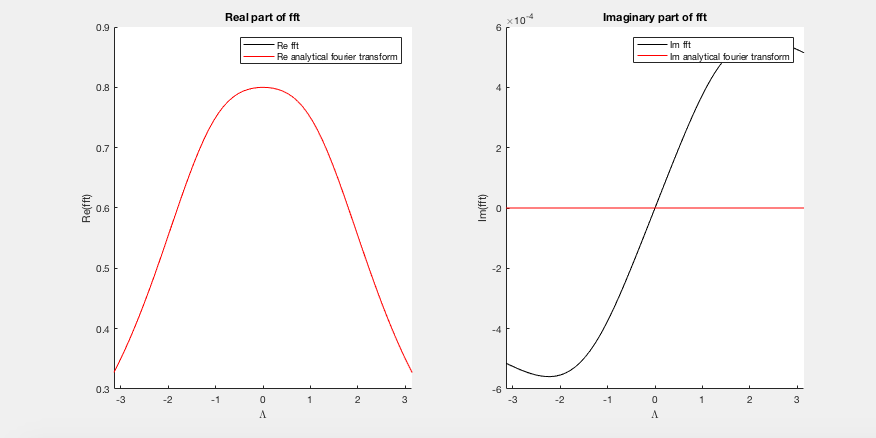
\includegraphics[width=\textwidth]{f1fig1}
            \label{pic:f1:1}
        \end{figure} \\
        Вещественные части графиков аналитического преобразования и вычисленной аппроксимации практически совпадают, а погрешность во мнимой части сравнима с величиной
        шага дискретизации \texttt{step}.
        \clearpage
        \item
        Сразу после построения предыдущего графика, вызовем \texttt{plotFT} с тем же параметром hFigure и следующим набором параметров:\\
        \texttt{step} = \(10^{-2}\), \texttt{inpLimVec} = \( [-20, 30] \), \texttt{outLimVec} = \( [] \)
        \begin{figure}[!h]
            \centering
            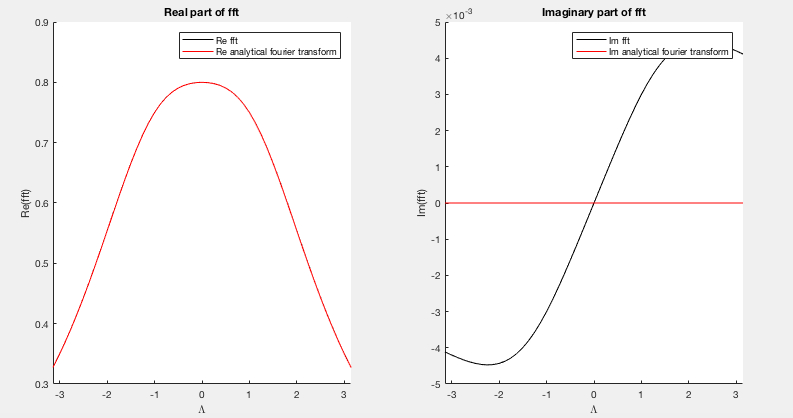
\includegraphics[width=\textwidth]{f1fig2}
            \label{pic:f1:2}
        \end{figure} \\
        Несмотря на несимметричное окно \texttt{inpLimVec}, графики вещественных частей по-прежнему совпадают, 
        а мнимых ~--- различаются на величину порядка \texttt{step}. Отметим, что, так как был передан пустой вектор \texttt{outLimVec}, то пределы 
        по оси абсцисс~\(\lambda\) на графиках не изменились.
        \clearpage
        \item
        \texttt{step} = \(10^{-5}\), \texttt{inpLimVec} = \( [-10, 20] \), \texttt{outLimVec} = \( [-2\pi, \pi] \)
        \begin{figure}[!h]
            \centering
            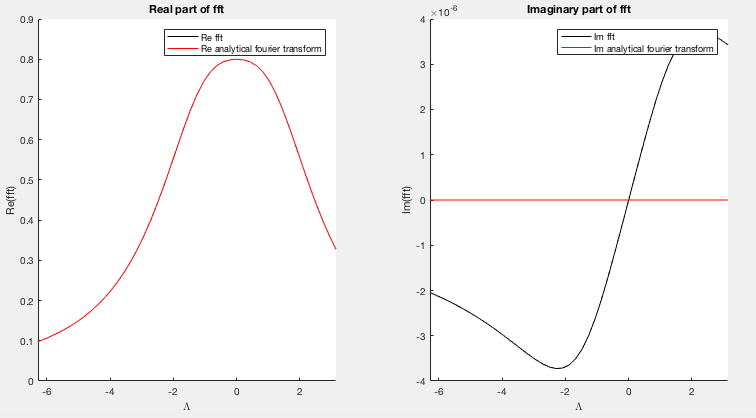
\includegraphics[width=\linewidth]{f1fig3}
            \label{pic:f1:3}
        \end{figure} \\
        В данном случае используется несимметричное окно для вывода (\texttt{outLimVec})
        \setcounter{icount}{\value{enumi}}
    \end{enumerate}
    Кроме того, на примере данной функции проиллюстрируем \emph{эффект наложения спектра (aliasing)}: для этого, отобразим на графике не только
    аналитическое преобразование Фурье, но и его же, сдвинутое влево и вправо на \(\frac{\pi}{\Delta t}\), где \(\Delta t\) = \texttt{step} 
    ~--- частота дискретизации. Из \cite{Roublev:fourier} известно, что численная аппроксимация \(\fft\) есть сумма аналитического преобразования 
    и сдвинутых аналитических преобразований \(\forall \lambda \in \left[-\frac{\pi}{\Delta t}, \frac{\pi}{\Delta t}\right] \).
    \clearpage
    \begin{enumerate}
        \setcounter{enumi}{\value{icount}}
        \item 
        \texttt{step} = \(1\), \texttt{inpLimVec} = \( [-20, 20] \), \texttt{outLimVec} = \( [\pi, \pi] \)
        \begin{figure}[!h]
            \centering
            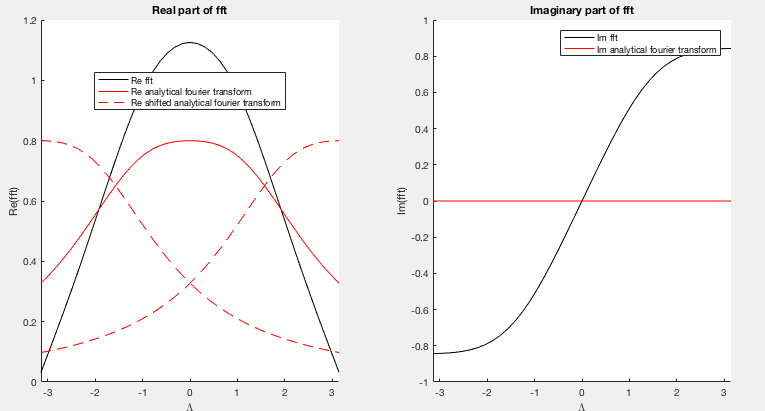
\includegraphics[width=\linewidth]{f1fig4}
            \label{pic:f1:4}
        \end{figure} \\
        Для преобразований Фурье \( \four \) ограниченного спектра \\ (таких, что \( \exists\Lambda \, \colon \four =0, \; \forall \lambda \colon |\lambda| > \Lambda \))
        из \cite{Roublev:fourier} известно, что эффект не будет проявляться при \(\Delta t \leqslant \Delta_{t}^\text{н}\),
        где \(\Delta_{t}^\text{н} = \frac{\pi}{\Lambda}\) ~--- так называемая частота Найквиста (Nyquist rate).
        Однако, в силу того, что спектр полученного аналитически преобразования Фурье \eqref{eq:fourier:f1} 
        неограничен (т.е. \(\not\exists\Lambda \, \colon \mathfrak{F_1}(\lambda) = 0, \; \forall \lambda \colon |\lambda| > \Lambda\)),
        полное устранение данного эффекта невозможно;
        но, т.к. аналитическое преобразование достаточно быстро стремится к нулю (со скоростью порядка \(\frac{1}{\lambda^2}\)), 
        то уменьшением шага дискретизации эффект наложения спектра можно свести к незначительному (см. \ref{it:noaliasing}).
        \clearpage
        \item
        \label{it:noaliasing}
        \texttt{step} = \(10^{-1}\), \texttt{inpLimVec} = \( [-20, 20] \), \texttt{outLimVec} = \( [\pi, \pi] \)
        \begin{figure}[!h]
            \centering
            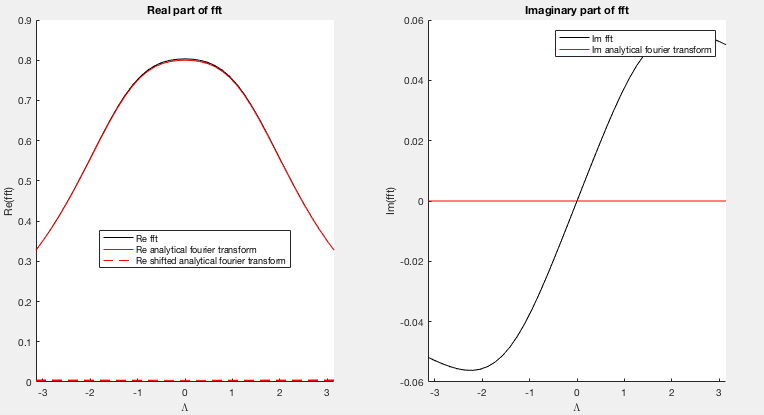
\includegraphics[width=\linewidth]{f1fig5}
            \label{pic:f1:5}
        \end{figure} \\
        Здесь хорошо видно, что, хотя эффект наложения спектра не устранён полностью, он практически незаметен, а сдвинутые части аналитического преобразования почти равны нулю.
    \end{enumerate}
    % subsection f1 (end)
    % section plotting (end)
    \clearpage
    \subsection{\(f_2(t) = \frac{e^{-|t|} - 1}{t} \)} % (fold)
    \label{sub:f2}
    Данная функция имеет разрыв типа "<скачок"> в точке 0,
    равно как и мнимая часть её преобразования Фурье~\eqref{eq:fourier:f2}:\\
    \begin{align*}
        \lim\limits_{t \rightarrow 0+0} f_2(t) &\not= \lim\limits_{t \rightarrow 0-0} f_2(t) \\
        \lim\limits_{\lambda \rightarrow 0+0} Im(\mathfrak{F_2}(\lambda))\,&\not=\,\lim\limits_{\lambda \rightarrow 0-0}\,Im(\mathfrak{F_2}(\lambda)
    \end{align*}
    \begin{enumerate}
        \item
        \label{it:noise}
        \texttt{step} = \(10^{-2}\), \texttt{inpLimVec} = \( [-10, 10] \), \texttt{outLimVec} = \( [-2\pi, 2\pi] \)
        \begin{figure}[!h]
            \centering
            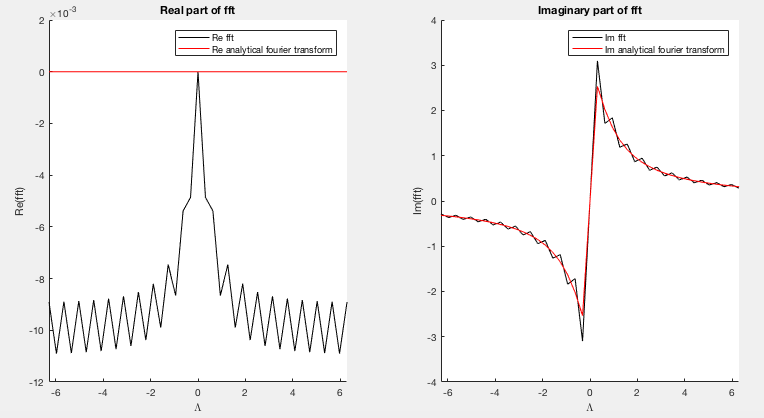
\includegraphics[width=\linewidth]{f2fig1}
            \label{pic:f2:1}
        \end{figure} \\
        Отклонение вещественной численной аппроксимации от аналитического значение есть величина порядка \texttt{step},
        а мнимые части графиков практически совпадают во всех точках.
        Заметим, что в точке 0 разрыва функции \(\mathfrak{F_2}\), а также в некоторых других точках непрерывности возникла \emph{рябь}.
        Её появление в точке разрыва первого рода обусловливается свойством преобразования Фурье разрывной функции из \cite{Roublev:fourier},
        а в некоторых точках непрерывности ~--- малым размером окна \([a, b]\) (\texttt{inpLimVec}).\\
        Устранить рябь в точке разрыва не представляется возможным, однако можно сгладить её в остальных точках, увеличив окно \texttt{inpLimVec}.
        \clearpage
        \item
        \label{it:lessnoise}
        \texttt{step} = \(10^{-2}\), \texttt{inpLimVec} = \( [-50, 50] \), \texttt{outLimVec} = \( [-2\pi, 2\pi] \)
        \begin{figure}[!h]
            \centering
            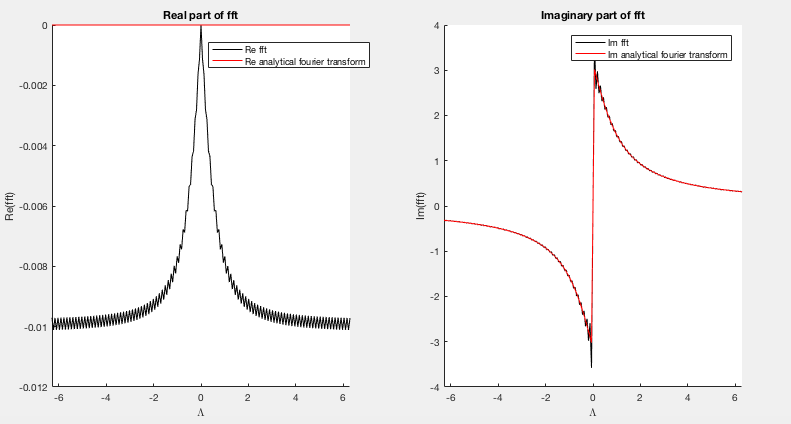
\includegraphics[width=\linewidth]{f2fig2}
            \label{pic:f2:2}
        \end{figure} \\
        Как можно видеть, размер ряби стал значительно меньше. Как и в предыдущем случае, отклонение вещественной части численной аппроксимации от аналитического значение
        есть величина порядка \texttt{step}.
        \clearpage
        \item
        \label{it:fftnoise}
        \texttt{step} = \(10^{-3}\), \texttt{inpLimVec} = \( [-10, 20] \), \texttt{outLimVec} = \( [-2\pi, 2\pi] \)
        \begin{figure}[!h]
            \centering
            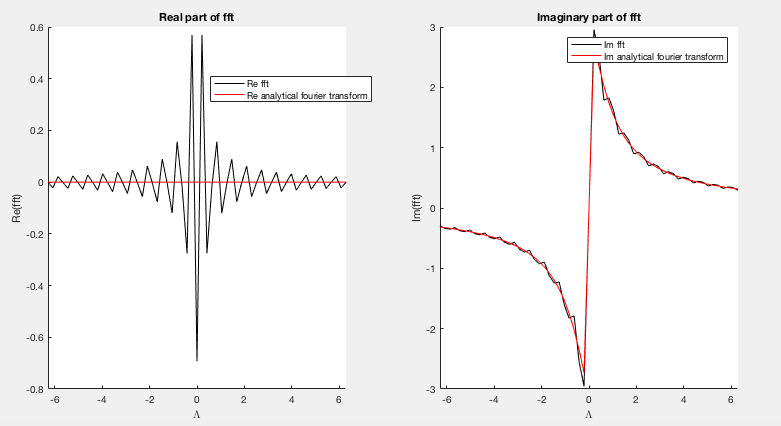
\includegraphics[width=\linewidth]{f2fig3}
            \label{pic:f2:3}
        \end{figure} \\
        В точке разрыва на графике вещественной части у численной аппроксимации наблюдается шум иного рода, порядка выше \texttt{step}; 
        это обусловливается особенностью работы функции \texttt{fft(\dots)} на несимметричном окне \([a, b]\) (\texttt{inpLimVec}).
    \end{enumerate}
    \clearpage
    % subsection f2 (end)
    \appendix
    \section{Код функции \texttt{plotFT}} % (fold)
    \label{lst:code}
    \begin{verbatim}
function [ res ] = plotFT( hFigure, fHandle, fFTHandle, ...
                            step, inpLimVec, outLimVec)
    res = struct('nPoints', [], 'Step', []);
    res.inpLimVec = inpLimVec;

    moe = .001;
    a = inpLimVec(1);
    b = inpLimVec(2);
    n = floor((b - a) ./ step) + 1;
    step = (b - a) ./ (n - 1);
    res.nPoints = n;
    res.Step = step;

    lsp = linspace(inpLimVec(1), inpLimVec(2), n);

    func = fHandle(lsp);

    fourier = step .* fftshift(fft(func));
    lsp = linspace(0, 2 * pi ./ step, n);

    lsp = lsp - lsp(floor(n ./ 2 + 1));  %symmetrical partition
    fourier = fourier .* exp(-1i.*lsp.*a) ; %shifting the fourier transform

    SPlotInfo = get(hFigure, 'UserData');

    if isempty(SPlotInfo)
        if isempty(outLimVec)
            limits = [0 0];
            for i = 1:n
                if abs(fourier(i)) > moe
                    if limits(1) == 0
                        limits(1) = i;
                    end
                    limits(2) = i;
                end
            end
            outLimVec = [lsp(limits(1)), lsp(limits(2))];
            res.outLimVec = outLimVec;
        end
    
        clf(hFigure); %clear figure window
    
        axRe = subplot(1, 2, 1);
        set(axRe, 'XLim', outLimVec);
        axRe.Title.String = 'Real part of fft';
        axRe.XLabel.String = '\Lambda';
        axRe.YLabel.String = 'Re(fft)';
    
        axIm = subplot(1, 2, 2);
        set(axIm, 'XLim', outLimVec);
        axIm.Title.String = 'Imaginary part of fft';
        axIm.XLabel.String = '\Lambda';
        axIm.YLabel.String = 'Im(fft)';
   
        SPlotInfo = struct('axRe', axRe, 'axIm', axIm);
    end

    if isempty(outLimVec)
        outLimVec = get(SPlotInfo.axRe, 'xLim');
    else
        set(SPlotInfo.axRe, 'XLim', outLimVec);
        set(SPlotInfo.axIm, 'XLim', outLimVec);
    end
    set(hFigure, 'UserData', SPlotInfo);

    % drawing graphs
    hFigure.CurrentAxes = SPlotInfo.axRe;
    hFigure.CurrentAxes.NextPlot = 'replacechildren';
    plot(lsp, real(fourier), 'Color', [0 0 0]); 
    legend('Re fft');
 
    if ~isempty(fFTHandle) 
        hFigure.CurrentAxes.NextPlot = 'add';
        plot(lsp, real(fFTHandle(lsp)), 'r');
        legend('Re fft', 'Re analytical fourier transform');
    end

    hFigure.CurrentAxes = SPlotInfo.axIm;
    hFigure.CurrentAxes.NextPlot = 'replacechildren';
    plot(lsp, imag(fourier), 'Color', [0 0 0]);
    legend('Im fft');

    if ~isempty(fFTHandle) 
        hFigure.CurrentAxes.NextPlot = 'add';
        plot(lsp, imag(fFTHandle(lsp)), 'r');
        legend('Im fft', 'Im analytical fourier transform');
    end
end
    \end{verbatim}
    % section code (end)
    \begin{thebibliography}{0}
        \addcontentsline{}{section}{Список литературы}
        \bibitem{Roublev:fourier} И. В.~Рублёв. Лекционный курс \emph{Преобразования Лапласа-Фурье},
        кафедра Системного~Анализа, Факультет Вычислительной Математики и Кибернетики, МГУ~им.~М.~В.~Ломоносова, 
        2017
        \bibitem{RoublevTochilin:matlab} И. В.~Рублёв, П. А.~Точилин. Лекционный курс \emph{Программирование на языке \texttt{MATLAB}},
        кафедра Системного~Анализа, Факультет Вычислительной Математики и Кибернетики, МГУ~им.~М.~В.~Ломоносова, 
        2017
        \bibitem{Matlab:help} Справочные средства языка \texttt{MATLAB}
    \end{thebibliography}
\end{document}
